\documentclass[12pt,a4paper]{article}

% --- Paquetes base (orden recomendado) ---
\usepackage[spanish,es-noshorthands]{babel}
\usepackage[utf8]{inputenc}
\usepackage[T1]{fontenc}
\usepackage{lmodern}
\usepackage{microtype}

\usepackage{geometry}
\geometry{margin=2.5cm}
\usepackage{setspace}
\usepackage{ragged2e}
\usepackage{fancyhdr}
\usepackage{hyperref}
\hypersetup{colorlinks=false}

% --- Tablas y columnas anchas ---
\usepackage{booktabs}
\usepackage{tabularx}
\usepackage{array}
\usepackage{makecell}
\usepackage[table]{xcolor}
\usepackage[section]{placeins}

\newcolumntype{Y}{>{\RaggedRight\arraybackslash}X}

% --- Diagramas ---
\usepackage{tikz}
\usetikzlibrary{arrows.meta,positioning,babel,fit,shapes.symbols,calc}
\definecolor{becaccent}{HTML}{E84E36}
\tikzset{
  block/.style={draw, rounded corners, align=center, minimum height=10mm, minimum width=32mm, inner sep=3pt},
}

% --- Imágenes y figuras
\usepackage{graphicx}
\usepackage{caption}
\usepackage{float}
\graphicspath{{figuras/}}

% --- Estilo de página: número centrado abajo ---
\pagestyle{fancy}
\fancyhf{}
\cfoot{\thepage}
\renewcommand{\headrulewidth}{0pt}
\renewcommand{\footrulewidth}{0pt}

% --- Datos de portada ---
\newcommand{\Universidad}{Universidad Andrés Bello}
\newcommand{\Materia}{Tecnologías Disruptivas}
\newcommand{\NRC}{8090}
\newcommand{\Profesor}{Álvaro Sánchez Colmenares}
\newcommand{\NombreCaso}{Caso de estudio — Seguridad en Smart Cities}

% Integrantes ordenados por apellido + correos
\newcommand{\Integrantes}{%
  \begin{tabular}{@{}l}
    \textbf{Gabriel Cuevas}\\[-2pt]
    \texttt{\href{mailto:g.cuevasortzar@uandresbello.edu}{g.cuevasortzar@uandresbello.edu}}\\[6pt]
    \textbf{Alfredo Fuentes}\\[-2pt]
    \texttt{\href{mailto:a.fuentesnavarrete@uandresbello.edu}{a.fuentesnavarrete@uandresbello.edu}}\\[6pt]
    \textbf{Felipe Ochoa}\\[-2pt]
    \texttt{\href{mailto:f.ochoajohn@uandresbello.edu}{f.ochoajohn@uandresbello.edu}}\\[6pt]
    \textbf{Alonso Rodrigo Urra Villagra}\\[-2pt]
    \texttt{\href{mailto:a.urravillagra@uandresbello.edu}{a.urravillagra@uandresbello.edu}}\\[6pt]
    \textbf{Antonia Valdebenito}\\[-2pt]
    \texttt{\href{mailto:a.valdebenitofuentes@uandresbello.edu}{a.valdebenitofuentes@uandresbello.edu}}
  \end{tabular}
}

\newcommand{\Fecha}{\today}

\begin{document}

% --- Portada (sin número) ---
\pagenumbering{gobble}
\begin{titlepage}
  \centering
  \vspace*{1cm}
  {\Large \Universidad\par}
  \vspace{3cm}
  {\LARGE\bfseries \NombreCaso\par}
  \vspace{1.5cm}
  {\large \Materia\ (\textbf{NRC:} \NRC)\par}
  \vspace{0.4cm}
  {\large \textbf{Profesor a cargo:} \Profesor\par}
  \vspace{2.2cm}
  {\large \textbf{Integrantes}\par}
  \vspace{0.3cm}
  {\large \Integrantes\par}
  \vfill
  {\large \Fecha\par}
\end{titlepage}

% --- Cuerpo del informe ---
\clearpage
\pagenumbering{arabic}
\setstretch{1.15}
\justifying

\section*{Contexto del caso — Seguridad}

La ciudad ficticia \textit{Nueva Aurora} enfrenta un rápido crecimiento poblacional y se encuentra en un proceso de transformación hacia una \textit{Smart City}. En el eje de seguridad ciudadana, el desafío principal se manifiesta en el aumento de robos y en la baja integración de cámaras y sensores a nivel urbano, situación que limita la prevención, la reacción oportuna y la trazabilidad de incidentes.

Ante este contexto, la ciudad evalúa la adopción de tecnologías propias de las ciudades inteligentes —entre ellas, Internet de las Cosas (IoT), Inteligencia Artificial (IA), Big Data, \textit{blockchain}, 5G y soluciones energéticas asociadas— como base para articular un ecosistema de seguridad más proactivo, interoperable y basado en datos. Estas capacidades tecnológicas se consideran habilitadoras para la detección temprana de eventos, la coordinación táctica y la rendición de cuentas, con énfasis en el uso de IA en cámaras urbanas y el despliegue de sensores distribuidos.

\section{Definición del problema y alcance}

\subsection*{Problemas prioritarios}
\textbf{P1. Robos en espacio público y comercio de alta afluencia.} La ciudad evidencia un aumento sostenido de delitos contra la propiedad en zonas céntricas y nodos de transporte, afectando a peatones y locales comerciales.

\textbf{P2. Baja integración operativa de cámaras y sensores urbanos.} La infraestructura de videovigilancia y sensorización existe de forma fragmentada, sin interoperabilidad suficiente para detección temprana, trazabilidad ni coordinación de respuesta.

\subsection*{Causas principales}
\begin{itemize}
    \item \textit{Fragmentación tecnológica}: parques de cámaras heterogéneos, protocolos manuales y ausencia de estándares de intercambio de datos.
    \item \textit{Ceguera situacional}: escasa analítica de video en tiempo real y cobertura desigual de sensores (iluminación, aforos, botonería de alerta).
    \item \textit{Procesos reactivos}: tiempos de verificación largos por falta de correlación automática de eventos y evidencias.
    \item \textit{Limitaciones de infraestructura urbana}: iluminación deficiente y mobiliario que dificulta líneas de visión en puntos críticos.
\end{itemize}

\subsection*{Consecuencias}
\begin{itemize}
    \item \textit{Impacto ciudadano}: aumento de victimización y disminución de la percepción de seguridad.
    \item \textit{Ineficiencias operativas}: respuesta tardía y uso subóptimo de recursos de patrullaje y atención de emergencias.
    \item \textit{Baja trazabilidad}: dificultades para esclarecer hechos por falta de evidencia unificada y cadena de custodia digital.
\end{itemize}

\subsection*{Alcance del proyecto (fase piloto)}
\textbf{Área geográfica}: distrito céntrico de alta concurrencia (aprox. 3--4 km\textsuperscript{2}), que incluye eje comercial, dos estaciones de transporte masivo y tres intersecciones críticas.\\
\textbf{Horizonte temporal}: 12 meses (3 meses diseño/instalación, 6 meses operación y ajuste, 3 meses evaluación).\\
\textbf{Cobertura funcional}: integración de videovigilancia y sensores urbanos existentes, analítica de video en tiempo real para detección de eventos de riesgo, y tablero operativo para coordinación interinstitucional.\\
\textbf{Procesos incluidos}: monitoreo preventivo, verificación de incidentes, despacho coordinado, preservación de evidencia digital y reportabilidad.

\subsection*{Fuera de alcance}
\begin{itemize}
    \item Reformas normativas o penales; reestructuración orgánica de fuerzas de orden.
    \item Vigilancia intrusiva en recintos privados o sin habilitación legal.
    \item Sustitución total de infraestructura existente fuera del polígono piloto.
\end{itemize}

\subsection*{Objetivos medibles (12 meses)}
\begin{itemize}
    \item Reducir en \(\geq 15\%\) los delitos contra la propiedad en el polígono piloto, respecto de la línea base.
    \item Disminuir en \(\geq 30\%\) el tiempo promedio de verificación y despacho ante eventos detectados.
    \item Alcanzar \(\geq 95\%\) de disponibilidad de la plataforma integrada (cámaras, sensores, analítica y tablero).
    \item Lograr que \(\geq 60\%\) de los incidentes relevantes sean \textit{detectados automáticamente} por analítica de video/sensores.
\end{itemize}

\subsection*{Restricciones y supuestos}
\begin{itemize}
    \item \textit{Legales y de privacidad}: tratamiento de datos personales sujeto a principios de finalidad, minimización y seguridad; difusión acotada de imágenes.
    \item \textit{Técnicas}: heterogeneidad de dispositivos; conectividad variable; necesidad de estándares abiertos (ONVIF, APIs seguras).
    \item \textit{Operativas}: coordinación interinstitucional y continuidad operativa 24/7 con personal capacitado.
\end{itemize}

\subsection*{Actores involucrados}
\begin{itemize}
    \item Municipio (gestión urbana y seguridad), centros de monitoreo y emergencia.
    \item Fuerzas de orden y equipos de respuesta (coordinación táctica y despacho).
    \item Comunidad y comercio local (canales de reporte y prevención situacional).
    \item Proveedores tecnológicos e integradores (infraestructura, software y soporte).
\end{itemize}

\subsection*{Riesgos y salvaguardas éticas}
\begin{itemize}
    \item \textit{Riesgos}: sesgos algorítmicos, vigilancia excesiva, ataques a la infraestructura, uso indebido de datos.
    \item \textit{Salvaguardas}: evaluación de impacto en privacidad, anonimización cuando corresponda, controles de acceso y auditoría, cifrado extremo a extremo, políticas de retención y uso proporcional de la información.
\end{itemize}

\newpage
\section{Mapa de problemas (Causa - Consecuencias)}

\subsection*{Problema 1: Robos en vía pública}
\textbf{Robos en vía pública} en zonas de alta influencia y nodos de transporte, con afectación directa a peatones y comercios. Véase la figura \ref{fig:mapa-problemas-seguridad}.
\begin{figure}[htbp]
  \centering
  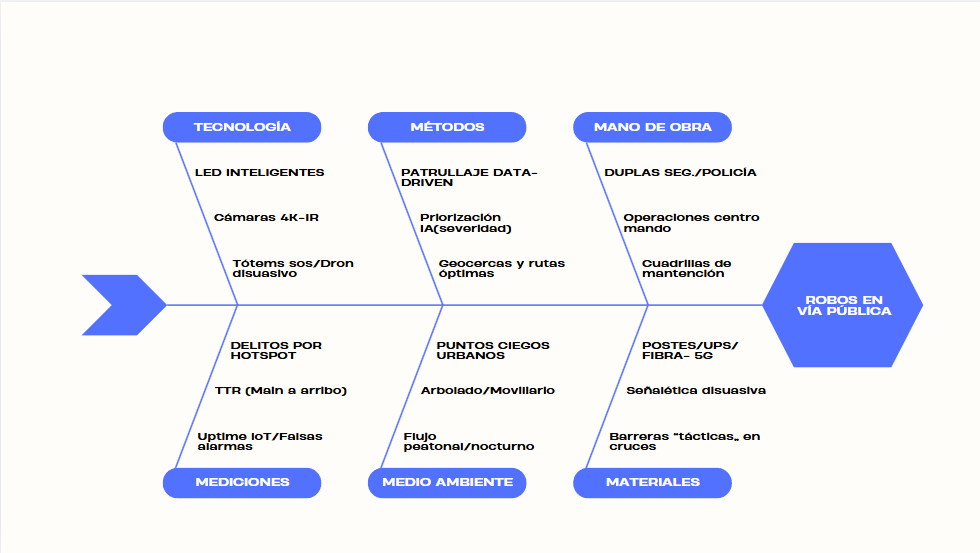
\includegraphics[width=\linewidth, keepaspectratio]{ishikawa_p1.png}
  \caption{Diagrama de Ishikawa del problema \textit{Robos en vía pública}.}
  \label{fig:mapa-problemas-seguridad}
\end{figure}

\subsection*{Causas inmediatas}
\begin{itemize}
    \item \textit{Fragmentación tecnológica}: Cámaras y sensores heterogéneos, con baja interoperabilidad y flujos manuales.
    \item \textit{Ceguera situacional}: Analítica de video limitada para detección temprana de eventos y cobertura desigual de sensorización.
    \item \textit{Procesos reactivos}: Verificación lenta por falta de correlación automática de alertas y evidencias.
    \item \textit{Infraestructura urbana subóptima}: Iluminación deficiente, mobiliario y arbolado que generan puntos ciegos.
\end{itemize}

\subsection*{Causas subyacentes}
\begin{itemize}
    \item \textit{Estándares y gobierno de datos insuficientes}: ausencia de APIs y protocolos abiertos para intercambio seguro.
    \item \textit{Capacidades operativas dispares}: roles, turnos y procedimientos no unificados entre vigilancia, monitoreo y despacho.
    \item \textit{Conectividad irregular}: tramos sin fibra/5G y respaldo eléctrico limitado que afectan la disponibilidad de equipos.
    \item \textit{Mantenimiento correctivo predominante}: fallas recurrentes y tiempos de reparación prolongados.
\end{itemize}

\subsection*{Consecuencias}
\begin{itemize}
    \item \textit{Impacto ciudadano}: Mayor victimización y disminución de la percepción de seguridad.
    \item \textit{Ineficiencias operativas}: Respuesta tardía y uso subóptimo de recursos de patrullaje y emergencia.
    \item \textit{Baja trazabilidad}: Dificultad para esclarecer hechos por carencia de evidencia integrada y cadena de custodia digital.
    \item \textit{Costos socioeconómicos}: Pérdidas para el comercio local y reducción de actividad en zonas críticas.
\end{itemize}

\subsection*{Relación causa–efecto (síntesis)}
\begin{table}[htbp]
\centering
\caption{Vinculación de causas con efectos del problema “Robos en vía pública”.}
\begin{tabular}{p{0.30\linewidth} p{0.36\linewidth} p{0.28\linewidth}}
\hline
\textbf{Categoría de causa} & \textbf{Evidencia/manifestación típica} & \textbf{Efecto principal} \\
\hline
Tecnología & Heterogeneidad de cámaras/sensores; sin correlación automática & Verificación lenta; baja detección temprana \\
Métodos & Patrullaje no dirigido por datos; rutas subóptimas & Cobertura reactiva; menor disuasión \\
Mano de obra & Roles/protocolos no unificados; capacitación desigual & Coordinación limitada en incidentes \\
Materiales & Iluminación insuficiente; señalética disuasiva escasa & Puntos ciegos y mayor oportunidad delictiva \\
Medio ambiente & Arbolado/mobiliario obstruyen; flujos peatonales desbalanceados & Zonas de riesgo persistentes \\
Mediciones & Falta de KPIs operativos; alto nivel de falsas alarmas & Mejora continua limitada \\
\hline
\end{tabular}
\end{table}

\subsection*{Indicadores asociados (línea base y metas)}
\begin{itemize}
    \item \textbf{Tasa de delitos contra la propiedad} (por 10\,000 hab.) en el polígono piloto: reducción relativa de \(\geq 15\%\) a 12 meses respecto de la línea base.
    \item \textbf{Tiempo medio de verificación y despacho (TTR)} desde la alerta hasta el envío de recurso: disminución de \(\geq 30\%\).
    \item \textbf{Disponibilidad de la plataforma integrada} (cámaras, sensores, analítica y tablero): \(\geq 95\%\).
    \item \textbf{Detección automática de incidentes relevantes} (analítica de video/sensores): \(\geq 60\%\) del total de incidentes registrados.
    \item \textbf{Tasa de falsas alarmas}: reducción a \(\leq 10\%\) mediante calibración y verificación.
\end{itemize}

\subsection*{Supuestos críticos}
\begin{itemize}
    \item Disponibilidad de conectividad (fibra/5G) y respaldo energético en puntos críticos.
    \item Acceso legal y seguro a datos para fines de prevención, reacción y trazabilidad, con políticas de minimización y retención.
    \item Coordinación interinstitucional efectiva para operación 24/7 y mantenimiento preventivo.
\end{itemize}

\subsection*{Problema 2: Baja integración operativa de cámaras y sensores}

\noindent La infraestructura de videovigilancia y sensorización urbana opera de forma fragmentada, con dispositivos heterogéneos y flujos de datos dispares. La ausencia de interoperabilidad y estandarización limita la detección temprana, la trazabilidad de incidentes y la coordinación de la respuesta.

\begin{figure}[htbp]
  \centering
  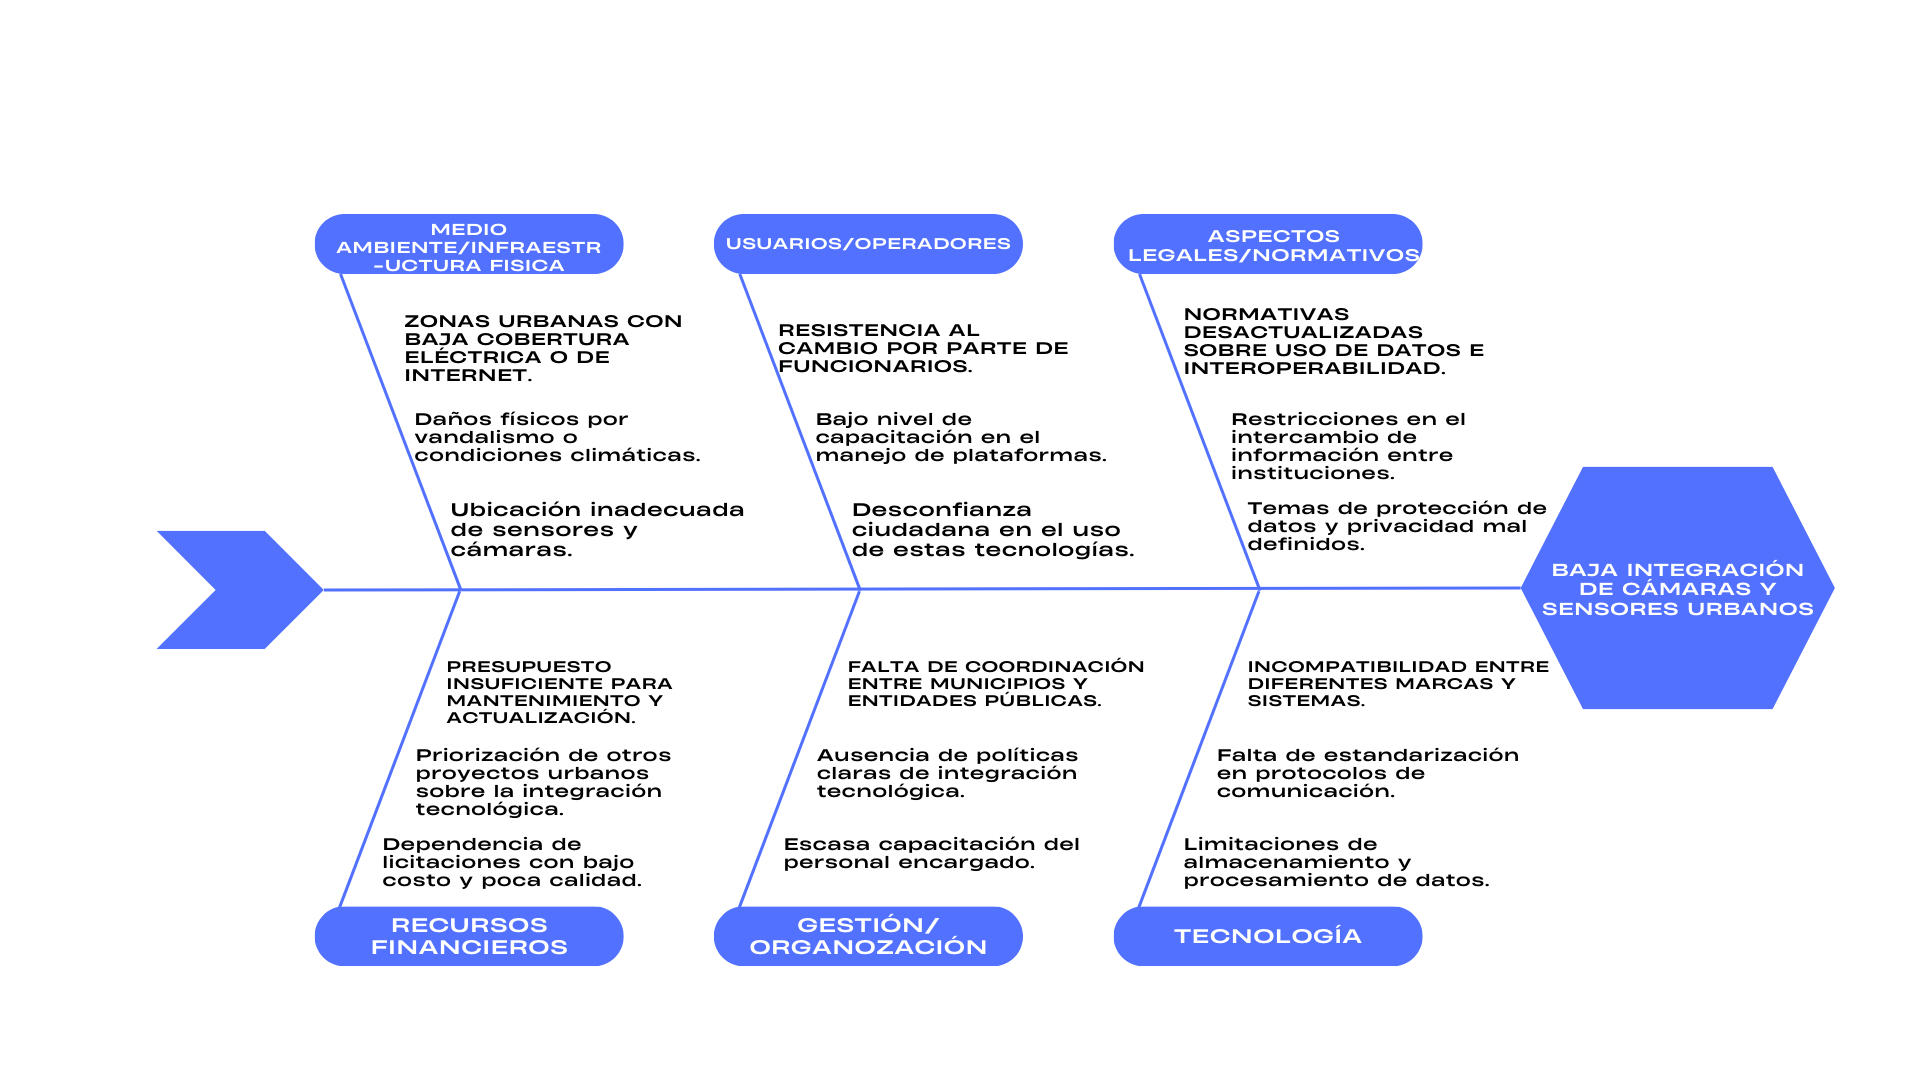
\includegraphics[width=\linewidth]{ishikawa_p2.png}
  \caption{Diagrama de Ishikawa — Problema 2: Baja integración operativa de cámaras y sensores.}
  \label{fig:ishikawa-p2}
\end{figure}

\subsection*{Causas e impactos (síntesis)}
\begin{table}[htbp]
\centering
\caption{Vinculación de causas con efectos del problema “Baja integración operativa”.}
\begin{tabular}{p{0.30\linewidth} p{0.36\linewidth} p{0.28\linewidth}}
\hline
\textbf{Categoría de causa} & \textbf{Evidencia/manifestación típica} & \textbf{Efecto principal} \\
\hline
Tecnología & Sistemas heterogéneos, sin perfiles ONVIF ni APIs alineadas & Imposibilidad de correlación; mayor latencia \\
Métodos & Verificación manual y scripts ad-hoc & Variabilidad operativa; tiempos de respuesta altos \\
Mano de obra & Capacitación dispar; dependencia del operador & Mayor tasa de error y falsas alarmas \\
Materiales & Falta de respaldo eléctrico y racks adecuados & Caídas de servicio; pérdida de datos \\
Medio ambiente & Interferencias/saturación en tramos inalámbricos & Pérdida de paquetes; \textit{jitter} en video/eventos \\
Mediciones & Sin KPIs ni telemetría de salud & Mejora continua limitada; fallas no detectadas \\
\hline
\end{tabular}
\end{table}

\subsection*{Indicadores asociados (línea base y metas)}
\begin{itemize}
    \item \textbf{Cobertura integrada} (\% de cámaras/sensores gestionados desde la plataforma): meta \(\geq 85\%\).
    \item \textbf{Latencia de ingestión y correlación}: tiempo desde evento a alerta unificada; meta \(\leq 5\) s en críticos.
    \item \textbf{Incidentes con correlación automática}: proporción con video, georreferencia y recurso vinculado; meta \(\geq 70\%\).
    \item \textbf{Disponibilidad del servicio de integración}: meta \(\geq 99.5\%\) mensual.
    \item \textbf{Tasa de falsas alarmas}: meta \(\leq 10\%\).
\end{itemize}

\subsection*{Supuestos críticos}
\begin{itemize}
    \item Disponibilidad de enlaces confiables (fibra/5G) y respaldo energético en sitios críticos.
    \item Acceso legal a flujos de datos para prevención, reacción y trazabilidad, con principios de minimización y seguridad.
    \item Inventario técnico actualizado (modelos, firmware, topología) y adopción de estándares de interoperabilidad.
    \item Coordinación operativa 24/7 y mantenimiento preventivo programado.
\end{itemize}

% ----------------------- MEJORA DE BENCHMARK NUMÉRICO -----------------------
\section{Ciudad referente}
\subsection*{1. Ciudad estudiada}
\textbf{Barcelona, España.} Pionera en arquitectura digital urbana, plataforma IoT \textit{Sentilo} y despliegues de sensorización, alumbrado y videovigilancia.

\subsection*{2. Tecnología concreta aplicada}
Plataforma urbana basada en estándares abiertos (\textit{Sentilo}) que integra:
\begin{itemize}
  \item Red de \textit{CCTV} con cámaras IP y perfiles ONVIF, enlazada a centros de control operativos.
  \item Sensores urbanos (iluminación telegestionada, aforo, acústica, calidad de aire, riego).
  \item Analítica en tiempo real y tableros geoespaciales para correlación evento--ubicación--recurso.
  \item Conectividad sobre fibra y redes móviles; telemetría de salud para garantizar disponibilidad.
\end{itemize}
\noindent(\textit{Base tecnológica:} \cite{sentiloCaseStudy,ciscoBarcelona})

\subsection*{3. Resultados medibles reportados (benchmark)}
\begin{itemize}
  \item \textbf{Ahorro energético en alumbrado público:} \(\sim 30\%\) de reducción del consumo gracias a LED + telegestión en el sistema urbano de iluminación \cite{harvardAsh}. 
  \item \textbf{Gestión del agua:} reportes de ahorro del orden de \(\sim\)US\$58 millones por iniciativas IoT (p.\,ej., riego inteligente, medición y control) \cite{harvardAsh}. 
  \item \textbf{Ingresos de estacionamiento:} incremento aproximado de \(\sim\)US\$50 millones/año atribuible a soluciones de \textit{smart parking} y gestión IoT \cite{harvardAsh}.
  \item \textbf{Magnitud del sistema de alumbrado y consumo:} >146\,000 puntos de luz; \(\sim 82{,}000\) MWh/año (\(\approx 20\%\) del consumo energético municipal), lo que contextualiza el potencial de ahorro por telegestión \cite{ajuntamentStreetLighting}. 
  \item \textbf{Evolución reciente:} plan de renovación para aumentar LED del 35\% al 50\% y avanzar hacia \textbf{gestión remota 100\%} del alumbrado \cite{ajuntamentRenewLighting}.
\end{itemize}

\subsection*{4. Desafíos o riesgos observados}
\begin{itemize}
  \item Interoperabilidad y dependencia de proveedores: exigir APIs abiertas y pruebas cruzadas (\cite{sentiloCaseStudy}).
  \item Continuidad operativa: vandalismo, energía y tramos con conectividad no redundada.
  \item Privacidad y ética: tratamiento proporcional de datos personales y mitigación de sesgos algorítmicos.
  \item Sostenibilidad: costos de mantenimiento/actualización y formación continua de operadores.
\end{itemize}

\subsection*{Adaptación al caso \textit{Nueva Aurora}}
\begin{itemize}
  \item \textbf{Línea base y KPIs:} medición inicial de delitos, TTR, falsas alarmas y disponibilidad, para contrastar reducciones/ahorros esperados siguiendo el enfoque de Barcelona.
  \item \textbf{Interoperabilidad desde la compra:} perfiles ONVIF, \textit{Sentilo}/APIs abiertas y pruebas de integración en licitaciones \cite{sentiloCaseStudy}.
  \item \textbf{Telegestión de iluminación:} adopción de LED + control punto a punto para perseguir ahorros cercanos a los observados (\(\sim 30\%\)) \cite{harvardAsh,ajuntamentStreetLighting}.
  \item \textbf{Riego inteligente y agua:} sensorización y control remoto de riego para replicar ahorros operacionales en agua \cite{ciscoBarcelona}.
\end{itemize}

\newpage
\section{Plan de implementación (pasos priorizados)}

\begin{table}[htbp]
\centering
\caption{Fases y entregables para materializar la propuesta.}
\begin{tabular}{p{0.10\linewidth} p{0.14\linewidth} p{0.46\linewidth} p{0.22\linewidth}}
\hline
\textbf{Fase} & \textbf{Periodo} & \textbf{Pasos priorizados} & \textbf{Entregables clave} \\
\hline
0 & Mes 1 &
Línea base (delitos, TTR, falsas alarmas); inventario técnico; polígono piloto; requisitos y pruebas de interoperabilidad en compras. &
Informe de línea base; pliego técnico; cronograma detallado. \\
\hline
1 & Meses 2--4 &
Gateway y bus de eventos; integración de \(\geq\)2 fabricantes por categoría; tablero mínimo viable; telemetría de salud; capacitación inicial. &
Plataforma MVP operativa; manuales iniciales; tablero v1. \\
\hline
2 & Meses 5--8 &
Analítica de video en tiempo real; motor de correlación; calibración para reducir falsas alarmas; procedimientos 24/7 y cadena de custodia. &
Modelos calibrados; SOPs 24/7; auditoría de evidencias. \\
\hline
3 & Meses 9--12 &
Escalamiento y \textit{hardening}; redundancia de conectividad/energía; formación avanzada; evaluación contra KPIs; plan de expansión. &
Informe de resultados; plan de mejora y escalamiento. \\
\hline
\end{tabular}
\end{table}

\section{Cuadro de gestión de recursos}

\begin{table}[htbp]
\centering
\caption{Recursos requeridos para el piloto y su gestión.}
\begin{tabular}{p{0.1\linewidth} p{0.40\linewidth} p{0.22\linewidth} p{0.20\linewidth}}
\hline
\textbf{Categoría} & \textbf{Descripción} & \textbf{Cantidad/Alcance} & \textbf{Responsable/Métrica} \\
\hline
Materiales & Postes, gabinetes, UPS/energía, racks, cableado y protecciones. & Según polígono (puntos críticos) & \textit{Uptime} energético; tiempo medio de reparación. \\
Equipos & Cámaras IP 4K-IR, sensores (botón, conteo, acústicos), switches PoE, gateways, servidores/almacenamiento. & \(\sim\)X cámaras, Y sensores, Z gateways & Disponibilidad por dispositivo; tasa de fallas/mes. \\
Tecnología & Bus de eventos, APIs, tablero unificado, analítica de video, observabilidad, IAM y seguridad. & Licencias/servicios + despliegue & Latencia \(\leq 5\) s; metadatos completos \(\geq 95\%\). \\
Personas & Jefatura de proyecto, arquitecto/integrador, ciberseguridad, analista/IA, operadores 24/7, mantenimiento, jurídico/datos. & Roles y turnos definidos & SLA de atención; cumplimiento SOP; auditorías OK. \\
\hline
\end{tabular}
\end{table}

\section{Impacto del proyecto en la ciudadanía}

\subsection*{Beneficios esperados}
\begin{itemize}
  \item \textbf{Seguridad y confianza}: detección y despacho más rápidos; mayor trazabilidad probatoria.
  \item \textbf{Calidad de vida}: reducción de falsas alarmas y patrullajes innecesarios; percepción de seguridad al alza.
  \item \textbf{Eficiencia pública}: mejor uso de recursos operativos; continuidad del comercio en zonas críticas.
  \item \textbf{Sostenibilidad}: menor huella por optimizar desplazamientos y telegestión de iluminación.
\end{itemize}

\subsection*{Indicadores de impacto (12 meses)}
\begin{itemize}
  \item \textbf{TTR verificación/ despacho}: reducción \(\geq 30\%\) en el polígono piloto.
  \item \textbf{Delitos contra la propiedad}: reducción relativa \(\geq 15\%\) vs. línea base.
  \item \textbf{Tasa de falsas alarmas}: \(\leq 10\%\) del total de alertas.
  \item \textbf{Percepción ciudadana}: mejora \(\geq 10\) p.p. en encuestas locales.
  \item \textbf{Disponibilidad de plataforma}: \(\geq 95\%\) (operativa integral).
\end{itemize}

\newpage
% --- Implementación del eje Seguridad ---------------------------------------
\section{Implementación del eje Seguridad}
\label{sec:impl-seguridad}

\subsection{Alcance y criterios de ubicación}
El despliegue se concentra en el polígono céntrico de Nueva Aurora, priorizando el \textbf{eje comercial}, las \textbf{estaciones Norte/Sur} y los \textbf{accesos viales}. La ubicación de cada dispositivo responde a: (i) afluencia peatonal/vehicular y reportes de incidentes, (ii) visibilidad y cobertura sin puntos ciegos, (iii) disponibilidad eléctrica y de postes/soportes, (iv) factibilidad de \textit{backhaul} (fibra/5G). La explicación siguiente referencia el mapa limpio (ver Fig.~\ref{fig:mapa-nueva-aurora}).

\begin{figure}[htbp]
  \centering
  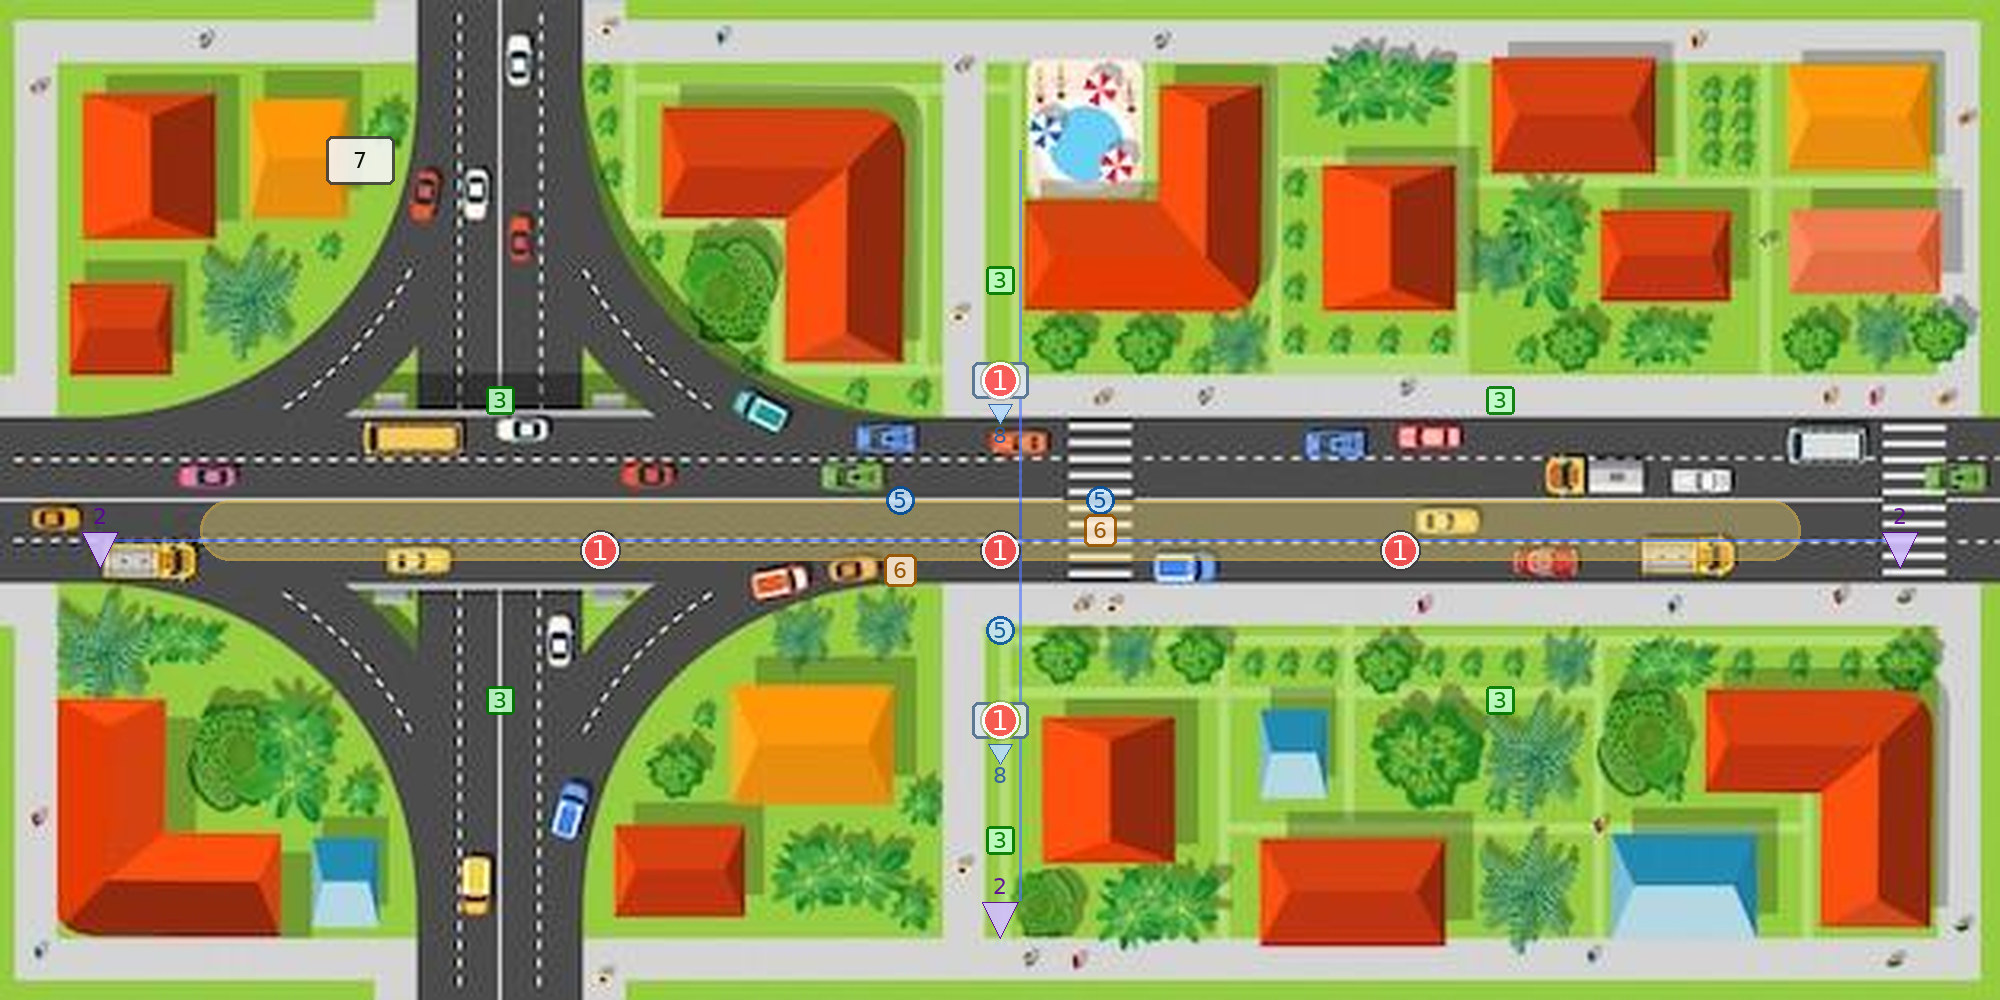
\includegraphics[width=\linewidth]{mapa-nueva-aurora.png}
  \caption{Mapa con puntos de control aplicados a las soluciones propuestas.}
  \label{fig:mapa-nueva-aurora}
\end{figure}

\subsection{Despliegue por componente (según marcadores del mapa)}
\begin{enumerate}
  \item \textbf{CCTV + IA (cruces y estaciones).} En los cruces A, B y C y en ambas estaciones se instalan cámaras fijas (cobertura de calzada y banquetas) y, donde aplique, una PTZ para seguimiento. Alimentación \textit{PoE} desde gabinetes cercanos; el \textbf{gateway/edge (6)} aplica analítica (merodeo, objetos abandonados, cruce en contrasentido) y envía eventos al COC (7). Se calibra zona/máscaras y se define repositorio/retención.
  \item \textbf{LPR/ANPR (accesos).} Cámaras de lectura de patentes en accesos oriente/poniente y salida sur, con iluminación IR y ángulo controlado. Generan metadatos (placa, fecha/hora, sentido) que se cruzan con alertas y listas de interés en el COC.
  \item \textbf{Botones de alerta SOS (paraderos/plazas).} Tótems con botón, cámara integrada, altavoz y baliza. Conexión \textit{PoE} o 5G; al activarse abren incidente en la consola del COC con \textbf{geolocalización} y previsualización de video.
  \item \textbf{Iluminación LED telegestionada (eje comercial).} Reemplazo/adecuación de luminarias por LED con control punto a punto (nodo NEMA/Zhaga y CMS). Escenas nocturnas con \textit{dimming} adaptativo (mayor nivel en cruces/paraderos), telemetría de fallas y base para sensores futuros.
  \item \textbf{Sensores acústicos (anomalías).} Malla de 2--3 nodos que triangulan eventos de \textbf{disparos/roturas} en el corredor. Disparan ticket automático con \textbf{verificación cruzada} en cámaras cercanas para reducir falsas alarmas.
  \item \textbf{Gateways/Edge (IoT/Video).} Gabinetes con \textit{switch} PoE, equipo industrial (CPU/GPU ligera) y \textbf{UPS}. Funciones: agregación de cámaras/sensores, \textit{buffering} local, analítica en borde y publicación de eventos (MQTT/REST) hacia la plataforma central.
  \item \textbf{COC -- Centro de Operaciones.} Sala con \textit{video wall}, VMS/analítica, CAD para despacho, gestión de evidencias (cadena de custodia), y panel de KPIs. Roles: operador 24/7, supervisor y analista. Protocolos de atención, escalamiento y privacidad.
  \item \textbf{Backhaul Fibra + 5G.} Tramo principal sobre el eje y vertical de refuerzo; arquitectura en \textbf{anillo} con \textit{switches} L2/L3 y VLAN de seguridad. 5G en estaciones como redundancia de subida; microondas donde la fibra no esté disponible.
\end{enumerate}

\subsection{Arquitectura y flujo de datos}
Dispositivo (1--5) \(\rightarrow\) \textbf{Edge (6)} (normalización/analítica/\textit{buffer}) \(\rightarrow\) \textbf{Backhaul (8)} \(\rightarrow\) \textbf{Plataforma} (VMS/EMS/CMS) \(\rightarrow\) \textbf{COC (7)} \(\rightarrow\) Despacho (policía/seguridad municipal). Se registran \textit{logs} y evidencias con control de acceso y auditoría.

\subsection{Operación, privacidad y mantenimiento}
\begin{itemize}
  \item \textbf{Operación:} monitoreo 24/7, verificación en \(\leq 2\) min, despacho coordinado, auditoría semanal de alarmas.
  \item \textbf{Privacidad:} señalética visible, enmascaramiento de zonas privadas, retención definida (p.\,ej., 15--30 días), control de accesos y registro de consultas.
  \item \textbf{Mantenimiento:} preventivo trimestral (limpieza ópticas, \textit{firmware}, recalibración analítica), correctivo con SLA, stock crítico de repuestos.
\end{itemize}

\subsection{Indicadores de éxito (KPI)}
\noindent \textit{Uptime} de plataforma y dispositivos; tiempo de detección, verificación y despacho; reducción de incidentes en zona priorizada; \% de falsas alarmas; incidentes resueltos con evidencia útil; ahorro energético por telegestión.

\section*{Glosario de Términos y Siglas}
\begin{description}
\item[APIs REST] Interfaces HTTP siguiendo principios REST.
\item[CCTV + IA] Videovigilancia con analítica inteligente.
\item[COC] Centro de Operaciones de Control.
\item[Gateways / Edge] Agregan y procesan datos localmente.
\item[IAM] Gestión de identidades y accesos.
\item[KPIs] Indicadores clave de rendimiento.
\item[LPR / ANPR] Reconocimiento automático de matrículas.
\item[ONVIF] Estándar de interoperabilidad en videovigilancia IP.
\item[QoS] Calidad de servicio de red.
\item[SLA] Acuerdo de nivel de servicio.
\item[TTR] Tiempo de resolución (o de verificación/ despacho, según se use).
\item[UPS] Sistema de alimentación ininterrumpida.
\end{description}

% ----------------------------- REFERENCIAS -----------------------------------
\section*{Referencias}
\begin{thebibliography}{99}

\bibitem{harvardAsh}
Adler, L. (2016, 18 de febrero).
\textit{How Smart City Barcelona Brought the Internet of Things to Life}.
Data-Smart City Solutions, Harvard Kennedy School.
Disponible en:
\url{https://datasmart.hks.harvard.edu/news/article/how-smart-city-barcelona-brought-the-internet-of-things-to-life-789}

\bibitem{ajuntamentStreetLighting}
Ajuntament de Barcelona (s.\,f.).
\textit{Street lighting management}.
Área de Urbanismo, Transición Ecológica, Servicios Urbanos y Vivienda.
Disponible en:
\url{https://ajuntament.barcelona.cat/ecologiaurbana/en/services/the-city-works/maintenance-of-public-areas/energy-management/street-lighting-management}

\bibitem{ajuntamentRenewLighting}
Ajuntament de Barcelona (2024, 14 de julio).
\textit{More work to renew and improve lighting in the city}.
Disponible en:
\url{https://www.barcelona.cat/infobarcelona/en/tema/urban-planning-and-infrastructures/more-work-to-renew-and-improve-lighting-in-the-city_1419476.html}

\bibitem{ciscoBarcelona}
Cisco (2015).
\textit{IoE-Driven Smart City Barcelona Initiative Cuts Water Bills, Increases Parking Revenues, and Creates Jobs}.
Perfil de jurisdicción.
Disponible en:
\url{https://www.cisco.com/c/dam/m/en_us/ioe/public_sector/pdfs/jurisdictions/Barcelona_Jurisdiction_Profile_final.pdf}

\bibitem{sentiloCaseStudy}
Bain, M. (2014).
\textit{Sentilo Case Study}.
Interoperable Europe.
Disponible en:
\url{https://interoperable-europe.ec.europa.eu/sites/default/files/document/2014-06/SENTILO%20case_joinup_v_1%202.pdf}

\end{thebibliography}

\end{document}
